\chapter{Extra-Credit Question}
\label{intro}

\textbf {Compute the Kendall Tau\textunderscore b score for both lists (use ``b'' because there will likely be tie values in the rankings).  Report both the Tau value and the ``p'' value.\\
See:\\}
{\url{http://stackoverflow.com/questions/2557863/measures-of-association-in-r-kendalls-tau-b-and-tau-c}}\\
{\url{http://en.wikipedia.org/wiki/Kendall_tau_rank_correlation_coefficient#Tau-b}}\\
{\url{http://en.wikipedia.org/wiki/Correlation_and_dependence}}\\ \\

\begin{itemize}
\item The Kendall Tau value is `0.926' and p value is `0.000217' for both the lists.
\item Below is the R code for calculating the Tau and p values.
\end{itemize}
\begin{figure}[h!]
\begin{center}
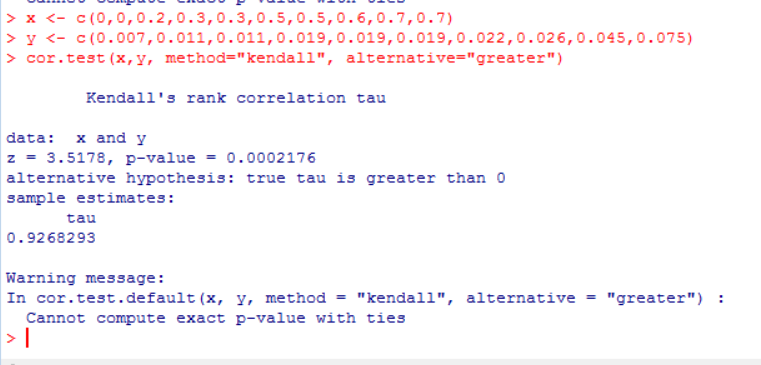
\includegraphics[scale=0.55, keepaspectratio=true]{figures/tau.PNG}
\caption{R code for calculating Tau and p values}
\label{fig:eqfig1}
\end{center}
\end{figure}
